\question{Действие сил пространственного заряда на траекторию крайнего электрона
  в плоском (ленточном) электронном потоке}

Рассмотрим движение электронов, сформированных в плоский электронный поток 
(рис.~\ref{img12.1}) в области, где на него не действуют никакие внешние силы, 
то есть внешние электрические или магнитные поля отсутствуют.

\begin{figure}[h!]
	\center
	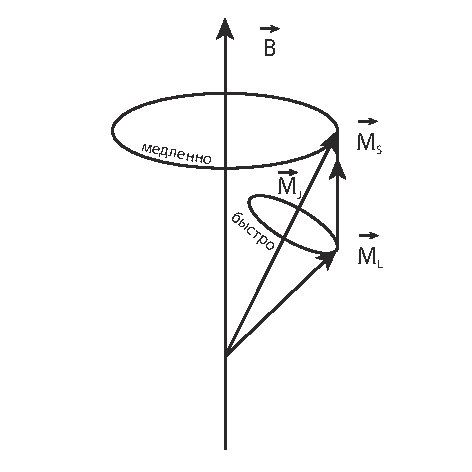
\includegraphics[width=.4\textwidth]{12_01}
	\caption{Схема плоского ленточного потока}
	\label{img12.1}
\end{figure}

Для упрощения задачи предположим, что толщина потока \( 2\D \) значительно 
меньше его ширины \( 2a \) и длины (вдоль оси 0z), а продольная скорость 
перемещения электронов вдоль оси 0z значительно меньше скорости света. Пусть 
задана объемная плоскость пространственного заряда \( \rho \). Тогда уравнение 
Пуассона \( \D U = -\rho / \Ez \) принимает вид
\begin{equation}
	\ppder{U}{x} + \ppder{U}{y} + \ppder{U}{z} = -\frac{\rho}{\eps_0}
	\label{eq12.3.2}
\end{equation}

Введенные ранее предположения позволяют утверждать, что изменение потенциала 
вдоль осей \( 0x \) и \( 0z \) значительно меньше изменения его вдоль 
\( 0y \). В этом случае уравнение (\ref{eq12.3.2}) преобразуется к виду
\begin{equation}
	\ppder{U}{y} = -\frac{\rho}{\eps_0}
	\label{eq12.3.3}
\end{equation}
 
Это приближение по существу означает замену пучка конечной ширины бесконечно 
широким, но суть физического процесса при этом не изменяется.

Для определения поля пространственного заряда можно использовать много 
методов. Наиболее простой заключается в использовании теоремы Гаусса. Из 
общего курса физики известно, что нормальная составляющая электрического поля 
(в данном случае -- \( E_y \)) для заряженной плоскости определяется
соотношением
\begin{equation}
	E_y = \frac{\sigma}{2\eps_0}
	\label{eq12.3.4}
\end{equation}
где \( \sigma = dq/dS \) поверхностная плотность пространственного заряда;
\( dS \) -- элемент площадки в плоскости \( x0z \).

Поскольку объемная плотность связана с зарядом соотношением 
\( \rho = dq/dV \), \( dV = 2\D ydS \) -- элемент объема, то из 
(\ref{eq12.3.4}) находим
\begin{equation}
	E_y = -\frac{\rho}{\eps_0}\D y
	\label{eq12.3.5}
\end{equation}
\( 2\D y \) -- толщина рассматриваемого электронного слоя.

Внутри потока \( \rho = const \), следовательно, поле на оси пучка равно нулю 
и линейно возрастает к его границам (рис. \ref{img12.2}).

\begin{figure}[h!]
	\center
	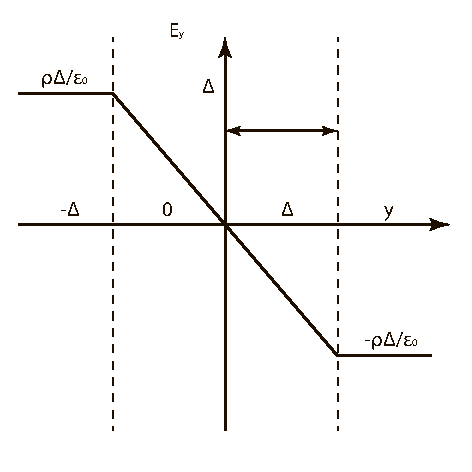
\includegraphics[width=.4\textwidth]{12_2}
	\caption{Зависимость распределения напряженности поля пространственного
		заряда от \( y \)}
	\label{img12.2}
\end{figure}
 
Рассмотрим теперь траектории электронов. Для этого следует воспользоваться 
классическим уравнением движения
\begin{equation}
	m\ddot{\vec{r}} = -e\vec{E}_0
	\label{eq12.3.6}
\end{equation}
где под \( E_0 = -\vec{j}E_0 \) следует понимать поле пространственного 
заряда. 

Векторное уравнение движения распадается на три скалярных:
\begin{equation}
	\ddot{y} = -\left| \frac{e}{m} \right|E_y; \quad
	\ddot{x} = \ddot{z} = 0
	\label{eq12.3.7}
\end{equation}

Если считать, что все электроны пучка в начальный момент (\( t = 0\)) имеют 
только составляющие  скорости вдоль \( y \) и \( z \) 
(\( \vec{v}_0 = \vec{j}v_{0y} + \vec{k}v_{0z} \)), причем 
\( |\vec{v}_0| = v_0 \approx v_{0z} \gg v_{0uy} \), то вдоль координаты 
\( x \) их положение не меняется: \( x = x_0 \). Движение электронов вдоль оси 
\( 0z \) описывается законом \( z = v_0 t \) (считаем, что все электроны 
влетают в плоскости \( z = 0 \) при \( t = 0 \)).

Продольная скорость электронов и плотность тока связаны соотношением
\begin{equation}
	j = -\rho v_0
	\label{eq12.3.8}
\end{equation}
Знак минус указывает на то, что это поток электронов. Для потока толщиной 
\( 2\D \) и шириной \( 2a \)
\begin{equation}
	j = \frac{I_0}{4a\D}
	\label{eq12.3.9}
\end{equation}
и из (\ref{eq12.3.5}) с учетом (\ref{eq12.3.9}) для граничных электронов (при 
\( y = \D \)) находим
\begin{equation}
	E_y = -\frac{I_0}{4a\eps_0 v_0} = 
		-\frac{1}{4\eps_0 a \sqrt{2\left|\frac{e}{m}\right|}}
		\frac{I_0}{U_0^{1/2}}
	\label{eq12.3.10}
\end{equation}

Уравнение (\ref{eq12.3.7}) в этом случае принимает вид:
\begin{equation}
	\ddot{y} = \left| \frac{e}{m} \right| \frac{I_0}{4a\eps_0 v_0}
	\label{eq12.3.11}
\end{equation}

Для определения вида траекторий лучше перейти к уравнению траекторий путем 
следующих замен:
\[
	\frac{dy}{dt} = \frac{dy}{dz}\frac{dz}{dt} = v_0 \frac{dy}{dz};\quad
	\frac{d^2 y}{dz^2} = v_0 \frac{d}{dz}\left( \frac{dy}{dz} \right)
		\frac{dz}{dt} = v^2_0 \frac{d^2 y}{dz^2}
\]
 
В результате
\begin{equation}
	\frac{d^2 y}{dz^2} = \left| \frac{e}{m} \right| \frac{I_0}{4av^3_0\eps_0}
	\label{eq12.3.12}
\end{equation}
Продольная скорость движения \( v_0 \) связана с ускоряющим потенциалом 
\( U_0 \) известным соотношением \( v_0 = \sqrt{2U_0\left| e/m \right|} \).
Подставляя это соотношение в (\ref{eq12.3.10}),  получаем: 
\( \ddot{y} = P\alpha \). Здесь введены постоянные 
\[ 
	\alpha = \left( 8\eps_0 a \sqrt{2\left| e/m \right|} \right)^{-1}
\]
и
\begin{equation}
	P = \frac{I_0}{U_0^{3/2}}
	\label{eq12.3.13}
\end{equation}
которую называют <<первеанс>> электронного потока. Интегрируя дважды по 
\( z \), находим решение в виде
\begin{equation}
	y(z) = y(0) + \tg\gamma_o z + \frac{1}{2}P\alpha z^2 
	\label{eq12.3.14}
\end{equation}
где \( \tg\gamma_0 = v_{0y}/v_0 \); \( \gamma_0 \) -- угол влета электрона в 
плоскости \( z = 0 \); \( y(0) \) -- начальная координата электрона (для 
граничного электрона -- \( y(0) = \D \)).
\begin{figure}[h!]
	\center
	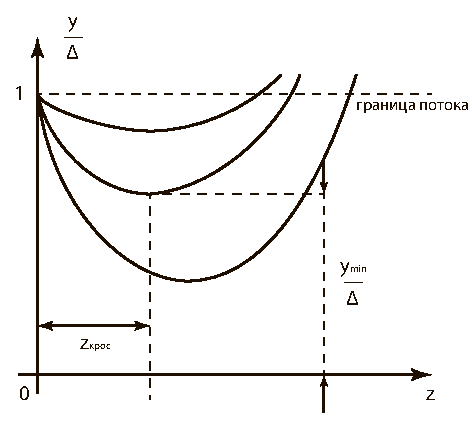
\includegraphics[width=.4\textwidth]{12_3}
	\caption{Контур ленточного потока при отсутствии внешних полей}
	\label{img12.3}
\end{figure}

Уравнение (\ref{eq12.3.14}) определяет контур электронного ленточного потока. 
Это -- парабола, вид которой определяется величиной \( \tg\gamma_0 \). При
\( \tg\gamma_0 < 0 \) (сходящийся поток), толщина потока сначала уменьшается 
(рис.~\ref{img12.2}), достигая минимума в плоскости
\begin{equation}
	z_\text{крос} = -\frac{\tg\gamma_0}{P\alpha}
	\label{eq12.3.15}
\end{equation}
 
При этом
\[
	y_{min} = \D\left[ 1 - \frac{\tg\gamma_0^2}{2P\alpha\D} \right]
\]
Затем поток начинает расширяться. Плоскость, где электронный пучок приобретает 
минимальную толщину, называется плоскостью кроссовера, а минимальная 
толщина -- кроссовер.